\documentclass[../../main.tex]{subfiles}

\begin{document}
\chapter{Manual de usuario}

% Introducción 
% Instalación
% Interfaz
% Proyectos
% Edición
% Búsqueda
% Compilación
% Terminal
% Configuración
% Atajos de Teclado
% FAQ

%% Seccion de Introducción     
\section{Introducción}
\textbf{SamaruC Retro Editor} es un entorno de desarrollo integrado (IDE) especializado para programación en lenguaje C, diseñado con una interfaz moderna y funcional basada en JavaFX.

\par{\textbf{Nota:} El nombre \textit{SamaruC} es un juego de palabras. Por una parte \textit{Samaruc} es un pez endémico de la Comunidad Valenciana en grave peligro de extinción, referenciando la región de origen del proyecto. Por otra parte, remarca la terminación con letra mayuscula de la \lstinline|C|, haciendo referencia al lenguaje de programación para el cual está optimizado este editor.}

\subsection{Características principales}
\begin{itemize}
    \item \textbf{Editor de código} con resaltado de sintaxis para C/C++.
    \item \textbf{Gestión de proyectos} con explorador de archivos integrado.
    \item \textbf{Compilación y ejecución} directa desde el IDE.
    \item \textbf{Terminal integrada} con consola de salida y depuración.
    \item \textbf{Búsqueda avanzada} en archivos y proyectos completos.
    \item \textbf{Pestañas múltiples} para trabajar con varios archivos simultáneamente.
    \item \textbf{Soporte multiidioma} (Español/Inglés).
    \item \textbf{Deshacer/Rehacer} con historial ilimitado.
    \item \textbf{Iconos FontAwesome 5} para una interfaz moderna.
\end{itemize}

\clearpage

%% Seccion de instalación
\section{Instalación}
\subsection{Requisitos del Sistema}
\begin{itemize}
    \item \textbf{Java:} JDK 17 o superior.
    \item \textbf{Maven:} 3.6 o superior (para compilar desde código fuente).
    \item \textbf{Compilador C:} GCC, Z88DK o GBDK (según tu proyecto).
    \item \textbf{Sistema Operativo:} Windows, Linux o macOS.
\end{itemize}

\subsection{Instalación desde Código Fuente}
Para compilar y ejecutar el editor desde el código fuente:
\begin{enumerate}
    \item Clona o descarga el repositorio del proyecto.
    \item Abre una terminal en el directorio del proyecto.
    \item Ejecuta los siguientes comandos:
\end{enumerate}

\begin{lstlisting}[language = Java]
mvn clean compile
mvn install
mvn javafx:run
\end{lstlisting}

\subsection{Instalación desde Ejecutable}
Si tienes el paquete ejecutable (.exe en Windows):
\begin{itemize}
    \item Extrae el archivo \lstinline|RetroEditor-win.zip|.
    \item Ejecuta \lstinline|RetroEditor.exe|.
    \item No requiere instalación de Java (incluye runtime embebido).
\end{itemize}

\clearpage

%sección de interfaz
\section{Interfaz}
\subsection{Descripción de la Interfaz}

\subsubsection{Barra de Menús}
La barra de menús se encuentra en la parte superior de la ventana como se puede apreciar en la captura \ref{fig:Menus} y contiene los siguientes menús principales:

\begin{figure}[!htb]
    \centering
    
\includegraphics[width=10cm]{aplicacion/Menus.png}
    \caption{Situación de los menús desplegables de la herramienta.}
    \label{fig:Menus}
\end{figure}

\par{ Funciones principales de cada menú: }
\begin{itemize}
    \item \textbf{Archivo:} Crear, abrir, guardar y cerrar archivos. 
    \item \textbf{Edición:} Deshacer, rehacer, cortar, copiar, pegar. 
    \item \textbf{Compilación:} Compilar y ejecutar el proyecto actual.
    \item \textbf{Configuración:} Ajustes de idioma, compilador y preferencias.
    \item \textbf{Ayuda:} Acceso a este manual y acerca de.
\end{itemize}

\clearpage

\subsubsection{Barra de Herramientas}
Como se puede ver en la captura de pantalla \ref{fig:BarraHerramientas}, otra manera de acceder rápido a las funciones elementales de la herramienta es mediante la barra de herramientas con iconos representativos de cada función:

\begin{figure}[!htb]
    \centering
    
\includegraphics[width=10cm]{aplicacion/Captura_barra_herramientas.png }
    \caption{Barra de herramientas con los iconos representativos de cada función.}
    \label{fig:BarraHerramientas}
\end{figure}

\par{La barra de herramientas proporciona acceso rápido a las funciones más utilizadas:}

\begin{itemize}
    \item \faFolderPlus\ \textbf{Nuevo Proyecto:} Abre el dialogo de creación de un nuevo proyecto.
    \item \faFolderOpen\ \textbf{Abrir Proyecto:} Abre un proyecto o archivo existente.
    \item \faFile\ \textbf{Nuevo:} Crea un archivo nuevo.
    \item \faSave\ \textbf{Guardar:} Guardar el archivo actual.
    \item \faTimes\ \textbf{Cerrar:} Cierra el archivo actual.
    \item \faUndo\ \textbf{Deshacer:} Desacer la última acción realizada.
    \item \faRedo\ \textbf{Rehacer:} Rehacer la última acción deshecha.
    \item \faSearch\ \textbf{Buscar en archivo:} Herramientas de búsqueda en el archivo actual.
    \item \faSearchPlus\ \textbf{Buscar en proyecto:} Herramientas de búsqueda en todo el proyecto.
    \item \faCut\ \textbf{Cortar:} Función para cortar un texto seleccionado.
    \item \faCopy\ \textbf{Copiar:} Función para copiar un texto seleccionado.
    \item \faPaste\ \textbf{Pegar:} Función de pegado de texto copiado o cortado.
    \item \faHammer\ \textbf{Compilar:} Construcción y compilación del código fuente.
    \item \faStop\ \textbf{Detener:} Detener la ejecución del código fuente.
    \item \faPlay\ \textbf{Ejecutar:} Construcción, compilación y ejecución del código fuente.
    \item \faCog\ \textbf{Configuración:} Acceso a preferencias y configuración.
    \item \faQuestionCircle\ \textbf{Ayuda - Manual:} Abre este manual de usuario.
\end{itemize}

\subsubsection{Panel del Explorador de Proyectos}

\par{Ubicado en el lado izquierdo de la interfaz \ref{fig:ExploradorProyectos}, este panel muestra la estructura de directorios y archivos del proyecto activo.}

\begin{figure}[!htb]
    \centering
    
\includegraphics[width=7cm]{aplicacion/Area_explorador.jpg}
    \caption{Panel del explorador de proyectos.}
    \label{fig:ExploradorProyectos}
\end{figure}
\par{Desde este apartado es posible navegar por la jerarquía de carpetas, así como desplegar o contraer los directorios para visualizar u ocultar su contenido. Asimismo, los archivos pueden abrirse mediante doble clic, lo que permite visualizar y editar su contenido en el área de trabajo principal.}

\par{Al hacer clic con el botón derecho del ratón sobre esta zona, se despliega un menú contextual que ofrece opciones como la creación de un nuevo archivo o una nueva carpeta.}

\par{Si pulsamos la tecla \lstinline|Suprimir| con un archivo o carpeta seleccionada, aparecerá un diálogo de confirmación que si confirmamos eliminará el elemento seleccionado.}

\par{Además, tenemos un botón en la esquina superior izquierda del panel del explorador que permite refrescar la vista para mostrar los cambios realizados en el sistema de archivos, como la adición o eliminación de archivos fuera del editor.}

\clearpage

\subsubsection{Área de Edición con Pestañas}

\par{El área central donde se editan los archivos, como se puede ver en la captura \ref{fig:AreaEdicion}. Características:}

\begin{figure}[!htb]
    \centering
    
\includegraphics[width=10cm]{aplicacion/CapturaZonaEdicion.png}
    \caption{Área de edición con pestañas.}
    \label{fig:AreaEdicion}
\end{figure}

\begin{itemize}
    \item Soporte para múltiples archivos abiertos simultáneamente.
    \item Resaltado de sintaxis automático para C/C++.
    \item Numeración de líneas.
    \item Indicador de archivo modificado (*) en la pestaña.
\end{itemize}

 \subsubsection{Panel de Consola Y Monitor + Barra de Estado}

 \begin{figure}[!htb]
    \centering
    
\includegraphics[width=16cm]{aplicacion/ConsolaCaptura.jpg}
    \caption{Panel de consola y monitor.}
    \label{fig:PanelConsola}
\end{figure}

\begin{figure}[!htb]
    \centering
    
\includegraphics[width=16cm]{aplicacion/BarraEstadoCaptura.jpg}
    \caption{Barra de estado.}
    \label{fig:BarraEstado}
\end{figure}

 Este panel se divide en dos pestañas principales: \textbf{Consola} y \textbf{Monitor}, mostrados en las capturas \ref{fig:PanelConsola} y \ref{fig:BarraEstado} respectivamente, cada una con funciones específicas para la salida de compilación, ejecución y monitorización de la aplicación en tiempo real. Además, en la parte inferior de la ventana se encuentra la barra de estado que muestra el estado actual del editor.

\clearpage
%% TODO revisar y completar el contenido de cada sección a partir de aquí
\section{Gestión de Proyectos}

En esta sección se describen las herramientas para crear, abrir y organizar proyectos de programación en SamaruC Retro Editor \ref{fig:CrearNuevoProyecto}.

SamaruC Retro Editor utiliza una estructura de proyecto basada en directorios, donde cada proyecto corresponde a una carpeta que contiene los archivos fuente (.c), encabezados (.h) y otros recursos relacionados. El panel del explorador de proyectos permite gestionar esta estructura de manera visual e intuitiva.

\subsection{Crear un Nuevo Proyecto}

\begin{figure}[!htb]
    \centering
    
\includegraphics[width=12cm]{manual/Captura_manual_nuevo_proyecto.jpg}
    \caption{Crear un nuevo proyecto.}
    \label{fig:CrearNuevoProyecto}
\end{figure}

\begin{enumerate}
    \item Haz clic en el botón \textbf{Nuevo Proyecto} o usa el menú \textit{Archivo → Nuevo Proyecto}.
    \item Selecciona o crea una carpeta para el proyecto.
    \item El explorador mostrará la estructura del directorio.
    \item Comienza a crear archivos .c y .h.
\end{enumerate}

\clearpage 

\subsection{Abrir un Proyecto Existente}
A continuación se muestra el proceso para abrir un proyecto existente en SamaruC Retro Editor, como se puede apreciar en la captura de pantalla \ref{fig:AbrirProyectoExistente}.
\begin{figure}[!htb]
    \centering
    
\includegraphics[width=12cm]{manual/Captura_manual_abrir_proyecto.jpg}
    \caption{Abrir un proyecto existente.}
    \label{fig:AbrirProyectoExistente}
\end{figure}

\begin{enumerate}
    \item Haz clic en \textbf{Abrir Proyecto} o usa el menú \textit{Archivo → Abrir Proyecto}.
    \item Navega hasta la carpeta del proyecto.
    \item Selecciona el directorio raíz del proyecto.
    \item Todos los archivos del proyecto aparecerán en el explorador.
 \end{enumerate}

 \textbf{Consejo:} Organiza tus proyectos con subdirectorios (src/, include/, build/) para mejor estructura y mantenimiento.

 \subsection{Trabajar con Archivos}

 SamaruC Retro Editor permite crear, abrir, guardar y cerrar archivos de manera sencilla desde el menú de archivos o la barra de herramientas. Las operaciones básicas incluyen:
 
 \begin{itemize}
     \item \textbf{Crear archivo nuevo:} Botón ``Nuevo'' o \lstinline|Ctrl+N|.
     \item \textbf{Abrir archivo:} Doble clic en el explorador o botón ``Abrir''.
     \item \textbf{Guardar archivo:} \lstinline|Ctrl+S| o botón ``Guardar''.
     \item \textbf{Guardar como:} Menú \textit{Archivo → Guardar Como}.
     \item \textbf{Cerrar archivo:} Botón ``Cerrar'' o click en X de la pestaña.
 \end{itemize}

\clearpage 

\section{Edición de Código}

En esta sección se describen las herramientas y características disponibles para la edición de código fuente en SamaruC Retro Editor, incluyendo el resaltado de sintaxis, operaciones de edición y características avanzadas del editor.

\subsection{Resaltado de Sintaxis}

El editor de texto integrado en SamaruC Retro Editor utiliza la biblioteca RichTextFX para proporcionar resaltado de sintaxis automático para el lenguaje C. Esto facilita la lectura y escritura de código al diferenciar visualmente los distintos elementos del lenguaje como se puede ver en la captura de pantalla \ref{fig:ResaltadoSintaxis}.

\begin{figure}[!h]
    \centering
    
\includegraphics[width=8cm]{manual/Captura_manual_ejemplo_resaltado_sintaxis.jpg}
    \caption{Resaltado de sintaxis en el editor de código.}
    \label{fig:ResaltadoSintaxis}
\end{figure}



El editor proporciona resaltado automático para las siguientes categorías de elementos de código:

\begin{itemize}
     \item \textcolor{blue}{\textbf{Palabras clave:}} if, else, for, while, return, struct, etc.
     \item \textcolor{green}{\textbf{Comentarios:}} // comentarios de línea y /* bloques */.
     \item \textcolor{red}{\textbf{Cadenas:}} "texto entre comillas".
     \item \textcolor{teal}{\textbf{Números:}} 123, 0xFF, 3.14.
     \item \textcolor{brown}{\textbf{Funciones:}} printf, scanf, main.
     \item \textcolor{blue}{\textbf{Directivas:}} \#include, \#define, \#ifdef.
\end{itemize}

\clearpage 

\subsection{Operaciones de Edición}

En la siguiente tabla \ref{tab:atajos_teclado} se resumen las operaciones de edición más comunes y sus atajos de teclado correspondientes para mejorar la eficiencia al escribir código:

\begin{tabular}{|l|l|l|}
    \hline
    \textbf{Operación} & \textbf{Atajo} & \textbf{Descripción} \\
    \hline
    Deshacer & \lstinline|Ctrl+Z| & Revierte la última acción \\
    \hline
    Rehacer & \lstinline|Ctrl+Y| & Restaura la acción deshecha \\
    \hline
    Cortar & \lstinline|Ctrl+X| & Corta el texto seleccionado \\
    \hline
    Copiar & \lstinline|Ctrl+C| & Copia el texto seleccionado \\
    \hline
    Pegar & \lstinline|Ctrl+V| & Pega desde el portapapeles \\
    \hline
    Seleccionar todo & \lstinline|Ctrl+A| & Selecciona todo el texto \\
    \hline
\end{tabular}
\label{tab:atajos_teclado}

\subsection{Características Avanzadas}

SamaruC Retro Editor incluye varias características avanzadas para mejorar la experiencia de edición de código y la productividad del programador:
\begin{itemize}
     \item \textbf{Numeración de líneas:} Siempre visible para referencia.
     \item \textbf{Múltiples pestañas:} Trabaja con varios archivos simultáneamente.
     \item \textbf{Detección de cambios:} Asterisco (*) indica archivos modificados no guardados.
     \item \textbf{Historial ilimitado:} Deshacer/Rehacer sin límites.
\end{itemize}

\clearpage

\section{Búsqueda de Texto}

SamaruC Retro Editor ofrece potentes herramientas de búsqueda para localizar texto dentro de un archivo o en todo el proyecto. Estas funciones son esenciales para navegar rápidamente por el código, encontrar definiciones de funciones, referencias a variables o cualquier término específico.

\subsection{Buscar en Archivo Actual}

Cuando deseas buscar un término dentro del archivo que estás editando, puedes utilizar la función de búsqueda integrada de la siguiente manera:


\begin{itemize}
    \item Presiona \lstinline|Ctrl+F| o haz clic en el botón de búsqueda.
    \item Se abre un panel de búsqueda en la parte superior del editor.
    \item Escribe el término a buscar.
    \item Navega entre resultados con los botones Anterior/Siguiente.
\end{itemize}

\clearpage

\subsection{Buscar en Todo el Proyecto}

Si necesitas encontrar un término en todos los archivos de tu proyecto, la función de búsqueda en proyecto te permite hacerlo de manera eficiente como se detalla en las capturas de pantalla \ref{fig:BuscarEnProyecto} y \ref{fig:ResultadosBusquedaProyecto}.

\begin{figure}[!h]
    \centering
    
\includegraphics[width=8cm]{manual/Captura_manual_buscar_en_proyecto.jpg}
    \caption{Búsqueda en proyecto actual.}
    \label{fig:BuscarEnProyecto}
\end{figure}

\begin{itemize}
    \item Presiona \lstinline|Ctrl+H| o usa el botón \faSearch\ (\textbf{Buscar en proyecto}) en la barra de herramientas.
    \item Busca en todos los archivos del proyecto.
    \item Los resultados muestran archivo, línea y contexto.
    \item Haz doble clic en un resultado para abrir el archivo en esa ubicación.
\end{itemize}

\begin{figure}[!h]
    \centering
    
\includegraphics[width=6cm]{manual/Captura_manual_buscar_en_proyecto_resultados.jpg}
    \caption{Resultados de búsqueda en proyecto.}
    \label{fig:ResultadosBusquedaProyecto}
\end{figure}

\textbf{Consejo:} Usa la búsqueda en proyecto para encontrar definiciones de funciones, referencias a variables o identificar dónde se usa una función específica.

\clearpage





\subsection{Compilar el Proyecto}

Una vez abierto un proyecto, el entorno permite compilar automáticamente todos los archivos fuente utilizando la toolchain configurada. Durante este proceso, el sistema analiza el código, genera los binarios correspondientes y muestra información detallada sobre posibles errores o advertencias detectadas.

\begin{enumerate}
    \item Asegúrate de tener un proyecto abierto con archivos ``.c''.
    \item Haz clic en el botón \faHammer\ (\textbf{Compilar}) o usa el menú \textit{Compilación → Compilar}.
    \item La salida de compilación aparece en la consola inferior.
    \item Los errores y warnings se muestran con detalles de línea y archivo.
\end{enumerate}


\section{Compilación y Ejecución}

\subsection{Ejecutar el Programa}

Tras completar la compilación correctamente, la aplicación permite ejecutar el programa directamente desde el entorno de desarrollo. La salida estándar y la interacción con el usuario se realizan mediante la consola integrada, facilitando las pruebas rápidas durante el desarrollo.

\begin{enumerate}
    \item Después de compilar exitosamente, haz clic en el botón \faPlay\ (\textbf{Ejecutar}) o usa el menú \textit{Ejecución → Ejecutar}.
    \item El programa se ejecuta y la salida aparece en la consola.
    \item La entrada interactiva también está disponible en la consola.
\end{enumerate}

\textbf{Nota:} Es recomendable asegurarse de que el compilador se encuentre disponible en el PATH del sistema operativo. En caso contrario, la ruta completa al ejecutable puede configurarse manualmente desde las preferencias de la aplicación.

\clearpage

\section{Terminal y Consola}

\subsection{Consola de Salida}

La consola de salida centraliza toda la información relacionada con el proceso de compilación y ejecución del proyecto. Este panel permite al usuario supervisar el comportamiento del programa y detectar errores de forma rápida durante el desarrollo.

Muestra:

\begin{itemize}
    \item Salida del compilador (gcc, make, etc.).
    \item Mensajes de error y warnings.
    \item Salida del programa (stdout).
    \item Entrada interactiva (stdin).
\end{itemize}

\subsection{Consola de Depuración}

Además de la consola principal, el entorno incorpora una consola de depuración orientada al diagnóstico interno del IDE. Esta herramienta resulta útil para identificar problemas técnicos y analizar el comportamiento interno de la aplicación durante el desarrollo y las pruebas.

Registra:

\begin{itemize}
    \item Mensajes de log del sistema.
    \item Información de depuración del IDE.
    \item Errores internos y diagnósticos.
\end{itemize}

\subsection{Limpiar la Consola}

Con el objetivo de mantener una visualización más clara de la información, el entorno permite limpiar el contenido de la consola en cualquier momento. Esta función resulta especialmente útil tras varias ejecuciones consecutivas del programa.

Usa el botón de limpiar en el panel de consola para borrar la salida anterior y tener una vista limpia.

\clearpage

\section{Configuración y Personalización}

\subsection{Cómo abrir el diálogo de configuración}

La ventana de configuración centraliza las principales opciones de personalización y compilación del entorno. Puede abrirse en cualquier momento mediante el menú principal o desde la barra de herramientas.

Puedes acceder a ella de dos formas:

\begin{enumerate}
    \item Desde el menú principal: \textbf{Archivo  →  Configuración}.
    \item Desde la barra de herramientas: botón de \textbf{Configuración}.
\end{enumerate}

Podemos ver en la captura de pantalla \ref{fig:ConfigCompilador} la ventana de configuración con la pestaña de compilador activa:

\begin{figure}[!htb]
    \centering
    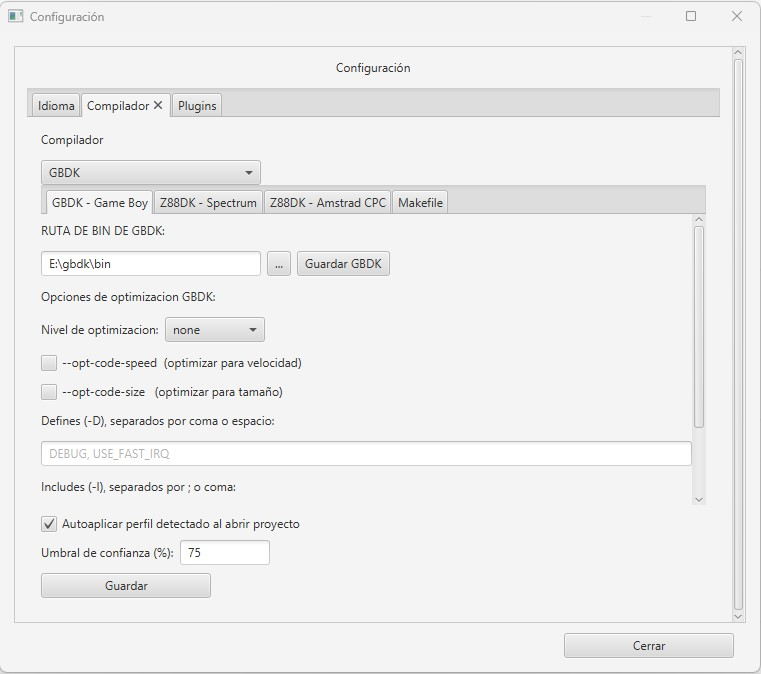
\includegraphics[width=10cm]{../imagenes/manual/Captura_config.jpg}
    \caption{Ventana de configuración con la pestaña de compilador activa.}
    \label{fig:ConfigCompilador}
\end{figure}


Al abrirse la ventana se muestran tres pestañas principales:

\begin{itemize}
    \item \textbf{Idioma}
    \item \textbf{Compilador}
    \item \textbf{Plugins}
\end{itemize}

En la parte inferior aparece el botón \textbf{Cerrar}. Además, la pestaña de compilador incorpora una zona de mensajes donde Samaruc muestra errores de validación y avisos relacionados con la configuración actual.

\subsection{Pestaña \texttt{Idioma}}

La pestaña \textbf{Idioma} agrupa las opciones relacionadas con la localización de la aplicación y la generación automática de documentación inicial para nuevos proyectos.

\subsubsection{Qué puedes cambiar}

Dentro de esta sección se muestran dos listas desplegables principales:

\begin{itemize}
    \item \textbf{Idioma de la interfaz}: cambia el idioma visible en menús, botones y textos de la aplicación.
    \item \textbf{Idioma del README para proyectos nuevos}: define en qué idioma se generará el \texttt{README.md} al crear un proyecto nuevo desde Samaruc.
\end{itemize}

Los valores disponibles actualmente son \textbf{Español} y \textbf{English}.

\clearpage

\subsection{Pestaña \texttt{Compilador}}

La pestaña está organizada en tres bloques:

\begin{enumerate}
    \item un selector superior con el compilador o flujo activo,
    \item un conjunto de subpestañas con opciones específicas,
    \item una zona inferior con preferencias de detección automática de perfil y el botón \textbf{Guardar configuración}.
\end{enumerate}

\subsubsection{Selector principal de compilador}

En la parte superior de la pestaña aparece una lista desplegable con cuatro opciones:

\begin{itemize}
    \item \textbf{GBDK}
    \item \textbf{Z88DK - Spectrum}
    \item \textbf{Z88DK - Amstrad CPC}
    \item \textbf{Makefile}
\end{itemize}

Este selector no solo cambia la subpestaña visible. También actualiza internamente el perfil activo que Samaruc utilizará para construir el proyecto.

\subsubsection{Qué implica cada opción}

\begin{description}
    \item[GBDK] Perfil orientado a proyectos de \textbf{Game Boy}. Al seleccionarlo, Samaruc considera este flujo como el principal y asocia internamente la ejecución con el emulador usado para Game Boy.
    \item[Z88DK - Spectrum] Perfil orientado a \textbf{ZX Spectrum}. Activa el modo \texttt{z88dk} con perfil \texttt{spectrum}.
    \item[Z88DK - Amstrad CPC] Perfil orientado a \textbf{Amstrad CPC}. Activa el modo \texttt{z88dk} con perfil \texttt{cpc}.
    \item[Makefile] Perfil genérico para proyectos que ya tienen su propia automatización de construcción.
\end{description}

Cambiar el selector superior puede persistir inmediatamente la selección del perfil. Aun así, si has modificado rutas o campos de texto, conviene terminar siempre pulsando \textbf{Guardar configuración}.

\subsubsection{Cómo guarda Samaruc la configuración}

Desde el punto de vista del usuario, hay dos formas de guardado dentro de esta pestaña:

\begin{itemize}
    \item \textbf{guardado inmediato en controles concretos}: algunos desplegables, casillas y botones secundarios guardan al interactuar con ellos.
    \item \textbf{guardado global}: el botón \textbf{Guardar configuración} valida el conjunto y deja persistido el perfil activo.
\end{itemize}

En la práctica, esto significa que puedes ver cambios que ya quedan almacenados incluso antes de pulsar el botón principal. Sin embargo, para evitar inconsistencias, la mejor rutina es:

\begin{enumerate}
    \item elegir el perfil.
    \item completar rutas y opciones.
    \item revisar mensajes de error si aparecen.
    \item pulsar \textbf{Guardar configuración} al final.
\end{enumerate}

\subsection{Subpestaña \texttt{GBDK}}

Esta subpestaña reúne la configuración específica para proyectos de Game Boy compilados con \texttt{GBDK}.

\subsubsection{Ruta de binarios}

Los primeros controles permiten indicar dónde está la carpeta \texttt{bin} de la toolchain. Si \textbf{GBDK} es el compilador activo, la ruta debe existir realmente. Si el campo está vacío o apunta a una carpeta inexistente, Samaruc no permitirá guardar la configuración completa.

\subsubsection{Nivel de optimización}

El campo \textbf{Nivel de optimización} ofrece estos valores admitidos:

\begin{description}
    \item[\texttt{none}] Sin optimización adicional. Puede ser útil al depurar o cuando quieres un comportamiento más predecible.
    \item[\texttt{-O1}] Optimización ligera. Buen punto de partida si buscas pocos cambios agresivos.
    \item[\texttt{-O2}] Nivel intermedio y normalmente razonable para uso general.
    \item[\texttt{-O3}] Optimización más intensa. Puede interesarte cuando priorizas rendimiento y ya has validado el proyecto.
\end{description}

\subsubsection{Casillas de optimización adicional}

Debajo del nivel aparecen dos opciones:

\begin{itemize}
    \item \textbf{--opt-code-speed}: orientada a velocidad.
    \item \textbf{--opt-code-size}: orientada a tamaño.
\end{itemize}

Estas casillas se guardan al pulsarlas. No son excluyentes a nivel de interfaz, así que conviene activarlas con criterio.

Si estás empezando con un proyecto, una estrategia práctica es usar primero un nivel simple como \texttt{-O1} o \texttt{-O2} y dejar desmarcadas las optimizaciones adicionales hasta tener una compilación estable.

\subsubsection{Campos de texto adicionales}

\begin{description}
    \item[Defines (-D)] Lista de símbolos de preprocesador. Puedes usar valores como \texttt{DEBUG}, \texttt{RELEASE} o cualquier macro propia del proyecto.
    \item[Includes (-I)] Rutas adicionales de cabeceras. El texto de ayuda indica separadores por coma o punto y coma.
    \item[Argumentos extra GBDK] Parámetros adicionales avanzados que quieras pasar a la toolchain.
\end{description}

\clearpage

\subsection{Subpestaña \texttt{Z88DK - Spectrum}}

Esta subpestaña está pensada para proyectos de \textbf{ZX Spectrum} compilados con \texttt{z88dk}.

\subsubsection{Ruta de binarios}

La parte superior funciona igual que en GBDK y está definida por un campo de ruta, botón \texttt{...} y botón \textbf{Guardar Z88DK}.

Si el perfil activo es \texttt{z88dk} para Spectrum, Samaruc exige que la ruta \texttt{bin} exista. Si no existe, el guardado global fallará.

\subsubsection{Selector \texttt{-clib}}

La opción \textbf{\texttt{-clib}} permite elegir la variante de biblioteca o runtime que se pasará a \texttt{z88dk}. Las opciones soportadas por la configuración actual son:

\begin{itemize}
    \item \texttt{none}.
    \item \texttt{default}.
    \item \texttt{noclib}.
    \item \texttt{ansi}.
    \item \texttt{new}.
    \item \texttt{sdcc\_ix}.
    \item \texttt{sdcc\_iy}.
    \item \texttt{clang\_ix}.
    \item \texttt{clang\_iy}.
\end{itemize}

Samaruc valida y normaliza este campo según la lista soportada por la aplicación. Si una configuración antigua contiene un valor no reconocido, la aplicación lo reconduce a un valor válido.

\subsubsection{Casilla \texttt{CRT\_ORG\_CODE=32768}}

La casilla \textbf{Usar \texttt{-pragma-define:CRT\_ORG\_CODE=32768}} permite activar esa directiva de compilación. En la configuración por defecto de Spectrum esta opción parte activada.

Úsala cuando tu proyecto o tu esquema de memoria espere ese origen. Si no estás seguro, conviene mantener el valor que usa tu proyecto actualmente.

\subsubsection{Campo \texttt{Target Z88DK}}

Este campo define el target de la plataforma y su valor habitual es \texttt{+zx}. El target debe empezar obligatoriamente por el carácter \texttt{+}. Si no empieza así, Samaruc mostrará un error y no guardará la configuración.

\subsubsection{Casilla \texttt{-create-app}}

La opción \textbf{Usar \texttt{-create-app}} indica a \texttt{z88dk} que genere la aplicación empaquetada. En la configuración por defecto de Spectrum esta casilla parte activada.

\subsubsection{Defines, Includes y argumentos extra}

Los tres campos finales permiten refinar el perfil:

\begin{itemize}
    \item \textbf{Defines (-D)} para macros de compilación.
    \item \textbf{Includes (-I)} para rutas adicionales.
    \item \textbf{Argumentos extra Z88DK} para parámetros avanzados.
\end{itemize}

\clearpage

\subsection{Subpestaña \texttt{Z88DK - Amstrad CPC}}

Esta subpestaña es equivalente a la anterior, pero aplicada al perfil de \textbf{Amstrad CPC}.

\subsubsection{Opción \texttt{-clib}}

Usa la misma lista de opciones admitidas que en Spectrum:

\begin{itemize}
    \item \texttt{none}.
    \item \texttt{default}.
    \item \texttt{noclib}.
    \item \texttt{ansi}.
    \item \texttt{new}.
    \item \texttt{sdcc\_ix}.
    \item \texttt{sdcc\_iy}.
    \item \texttt{clang\_ix}.
    \item \texttt{clang\_iy}.
\end{itemize}

\subsubsection{Casillas \texttt{CRT\_ORG\_CODE=32768} y \texttt{-create-app}}

En CPC estas opciones también están disponibles, pero en \texttt{CRT\_ORG\_CODE=32768} su valor por defecto en la configuración actual no coincide con Spectrum, en CPC parte desactivada.

\subsubsection{Campo \texttt{Target Z88DK}}

El valor habitual es \texttt{+cpc} y también aquí el campo debe empezar por \texttt{+} para que la validación sea correcta.

\subsubsection{Campos avanzados}

Como en Spectrum, dispones de \textbf{Defines (-D)}, \textbf{Includes (-I)} y \textbf{Argumentos extra Z88DK}.


\clearpage

\subsection{Subpestaña \texttt{Makefile}}

La opción \textbf{Makefile} está pensada para proyectos con un flujo de construcción propio.

\subsubsection{Campos disponibles en Makefile}

\begin{description}
    \item[Ejecutable make (opcional)] Permite indicar qué comando debe usarse para invocar \texttt{make}. Por ejemplo, \texttt{mingw32-make}.
    \item[Target para compilar] Si lo dejas vacío, Samaruc interpreta que debe usarse el target por defecto del \texttt{Makefile}.
    \item[Target para ejecutar] Si lo dejas vacío, Samaruc lo normaliza automáticamente a \texttt{run}.
    \item[Argumentos extra para make] Sirve para añadir parámetros adicionales, por ejemplo \texttt{-j4}.
\end{description}

\subsubsection{Normalización automática}

En esta subpestaña hay un detalle importante y es que el campo \textbf{Target para ejecutar} nunca se deja vacío al persistir, si no escribes nada, Samaruc lo transforma en \texttt{run}.

Las opciones de \texttt{Makefile} no admiten saltos de línea. Si pegas texto con retornos de carro o varias líneas, Samaruc lo rechazará y mostrará un error.

\subsubsection{Cuándo conviene usar Makefile}

Este perfil es recomendable cuando:

\begin{itemize}
    \item el proyecto ya trae su propio \texttt{Makefile}.
    \item no quieres adaptar la construcción a los perfiles integrados.
    \item necesitas un flujo más libre o más cercano al del proyecto original.
\end{itemize}

\clearpage

\subsection{Detección automática de perfil}

Debajo de las subpestañas aparece una sección adicional con dos controles:

\begin{itemize}
    \item \textbf{Autoaplicar perfil detectado al abrir proyecto}.
    \item \textbf{Umbral de confianza (\%)}.
\end{itemize}

\subsubsection{Autoaplicar perfil detectado}

Si esta casilla está activada, Samaruc puede cambiar automáticamente al perfil que considere más probable cuando abres un proyecto.

Si está desactivada, el campo de umbral queda deshabilitado en la interfaz.

\subsubsection{Umbral de confianza}

Este valor indica cuánta seguridad necesita Samaruc antes de aplicar automáticamente el cambio de perfil. El valor debe ser un entero entre \texttt{0} y \texttt{100}.

\begin{itemize}
    \item valores bajos: más automatización.
    \item valores altos: comportamiento más conservador.
    \item valor por defecto en la configuración actual: \texttt{75}.
\end{itemize}

Si introduces un valor no numérico o fuera del rango permitido, Samaruc mostrará un error y no guardará esta preferencia.

\clearpage

\subsection{Pestaña \texttt{Plugins}}

\subsubsection{Qué es la pestaña \texttt{Plugins}}

La pestaña \textbf{Plugins} es el lugar desde el que Samaruc permite gestionar extensiones externas. Está dividida en dos áreas principales:

\begin{enumerate}
    \item \textbf{plugins instalados localmente}.
    \item \textbf{marketplace de plugins} o catálogo remoto.
\end{enumerate}

En la primera área trabajas con plugins que ya están disponibles en la carpeta local de plugins. En la segunda, puedes consultar un catálogo remoto, ver información del plugin publicado e instalarlo directamente desde la red.

\subsubsection{Vista general de la pestaña}

En la siguiente tabla \ref{tab:resumen_plugins} se resumen las zonas principales de la pestaña \texttt{Plugins} y su función:
\begin{table}[!htb]
    \centering
    \begin{tabular}{|p{0.29\linewidth}|p{0.61\linewidth}|}
        \hline
        \textbf{Zona} & \textbf{Para qué sirve} \\
        \hline
        Lista de plugins instalados & Muestra los plugins detectados en la carpeta local de plugins. \\
        \hline
        Panel de acciones local & Permite instalar, habilitar, deshabilitar, eliminar, abrir carpeta y refrescar. \\
        \hline
        Indicador de recarga local & Muestra que Samaruc está recargando la lista de plugins. \\
        \hline
        Área de detalles del plugin & Enseña el nombre del JAR, su estado y las implementaciones detectadas. \\
        \hline
        Campo \textbf{URL catálogo} & Define qué dirección remota se usa como índice del marketplace. \\
        \hline
        Lista del marketplace & Muestra plugins publicados en el catálogo remoto. \\
        \hline
        Panel de acciones del marketplace & Permite actualizar el catálogo o instalar el plugin seleccionado. \\
        \hline
        Indicador de carga del marketplace & Señala que el catálogo remoto se está descargando o que un plugin se está instalando. \\
        \hline
        Área de detalles del marketplace & Muestra nombre, versión, autor, categoría, tamaño, verificación y descripción. \\
        \hline
    \end{tabular}
    
\end{table}
\label{tab:resumen_plugins}

\subsubsection{Bloque de plugins instalados}

La parte superior de la pestaña está dedicada a los plugins locales. Samaruc trabaja sobre archivos \texttt{.jar} situados en la carpeta \texttt{plugins} del entorno de trabajo.

La lista principal enseña cada JAR detectado junto a su estado. Normalmente verás algo parecido a esto:

\begin{itemize}
    \item \texttt{mi-plugin.jar (habilitado)}.
    \item \texttt{otro-plugin.jar (deshabilitado)}.
\end{itemize}

Al elegir un elemento de la lista, Samaruc rellena el panel de información con estos datos:

\begin{itemize}
    \item \textbf{Jar}: nombre del archivo.
    \item \textbf{Estado}: habilitado o deshabilitado.
    \item \textbf{Implementaciones}: nombres detectados dentro del JAR.
\end{itemize}

La lista trabaja sobre el archivo JAR y sobre las implementaciones de plugin que Samaruc puede descubrir dentro de él. Si un JAR está presente pero no contiene implementaciones válidas, la información mostrada puede ser limitada.

Debes tener en cuenta que solo se aceptan archivos \texttt{.jar} y que si ya existe un archivo con el mismo nombre, la copia puede sobrescribirlo.

\subsubsection{Bloque de marketplace}

La parte inferior de la pestaña está dedicada al marketplace remoto de plugins.

El marketplace funciona a partir de un \textbf{catálogo JSON remoto}. Ese catálogo contiene información sobre los plugins publicados y la URL desde la que puede descargarse cada uno.

Samaruc usa una URL por defecto, pero permite cambiarla desde la propia interfaz modificando el valor del campo \texttt{URL catálogo} y pulsando luego el botón \textbf{Guardar URL}. Si el campo está vacío o solo contiene espacios, Samaruc vuelve automáticamente a la URL por defecto del marketplace.

La lista del marketplace muestra plugins publicados en el catálogo remoto. Cada línea se construye con un formato sencillo:

\begin{itemize}
    \item nombre del plugin.
    \item versión entre paréntesis.
\end{itemize}


 \clearpage
 %% Seccion de miscelánea
\section{Miscelánea}

\subsection{Atajos de Teclado}

\par{Para mejorar la eficiencia y la experiencia de usuario, el editor incluye una serie de atajos de teclado para las funciones más comunes. Estos atajos permiten realizar acciones rápidamente sin necesidad de navegar por los menús, lo que agiliza el flujo de trabajo. A continuación se presenta la tabla \ref{tab:atajos_teclado_completa} con los atajos de teclado disponibles en \textbf{SamaruC Retro Editor}:}
\begin{table}[ht]
    \centering
    \small
    \begin{tabular}{p{3cm}p{6cm}}
        \toprule
            \textbf{Atajo} & \textbf{Acción} \\
        \midrule
            \lstinline|Ctrl+N| & Nuevo archivo \\
            \lstinline|Ctrl+O| & Abrir archivo \\
            \lstinline|Ctrl+S| & Guardar archivo \\
            \lstinline|Ctrl+W| & Cerrar archivo actual \\
            \lstinline|Ctrl+Z| & Deshacer \\
            \lstinline|Ctrl+Y| & Rehacer \\
            \lstinline|Ctrl+X| & Cortar \\
            \lstinline|Ctrl+C| & Copiar \\
            \lstinline|Ctrl+V| & Pegar \\
            \lstinline|Ctrl+A| & Seleccionar todo \\
            \lstinline|Ctrl+F| & Buscar en archivo actual \\
            \lstinline|Ctrl+H| & Buscar en proyecto completo \\
            \lstinline|F5| & Compilar proyecto \\
            \lstinline|F6| & Ejecutar programa \\
        \bottomrule
    \end{tabular}
    \caption{Atajos de teclado disponibles en SamaruC Retro Editor.}
    \label{tab:atajos_teclado_completa}
\end{table}

\subsection{Tecnologías utilizadas en el desarrollo de SamaruC Retro Editor:}
\begin{itemize}
    \item \textbf{JavaFX 17:} Framework de interfaz de usuario.
    \item \textbf{RichTextFX:} Editor de texto con resaltado de sintaxis.
    \item \textbf{Ikonli FontAwesome 5:} Iconos de interfaz.
    \item \textbf{Maven:} Gestión de dependencias y construcción.
\end{itemize}
\clearpage

\subsection{Requisitos del Sistema:}
\begin{itemize}
    \item Java 17+.
    \item 4 GB RAM mínimo (8 GB recomendado).
    \item 200 MB espacio en disco.
    \item Compilador C (Z88DK o GBDK).
\end{itemize}

\end{document}